\documentclass[11pt,titlepage,oneside,openany]{article}
\usepackage{times}

\usepackage[
	backend = biber,                		% Verweis auf biber
	language = auto,						% Sprache wird automatisch festgelegt
	style = authoryear,                	% Nummerierung der Quellen mit Zahlen
	maxcitenames=2,						% Number of authors before 
	bibencoding = utf8,						% UTF8 wird in biblatex aktiviert
	sorting = none,                 		% none = Sortierung nach der Erscheinung im Dokument
	sortcites = true,               		% Sortiert die Quellen innerhalb eines cite-Befehls
	block = space,                  		% Extra Leerzeichen zwischen Blocks
	hyperref = true,                		% Links sind klickbar auch in der Quelle
	doi=true,                      			% DOI anzeigen
	isbn=true,                     			% ISBN anzeigen
	alldates=year,                  		% Datum immer als DD.MM.YYYY anzeigen
	natbib=true,
	urldate=short                       % date in citations: https://tex.stackexchange.com/questions/89842/how-to-print-only-year-no-day-month-with-biblatex
]{biblatex}

% Define the bibtex file containing the references 
\addbibresource{references.bib}	


\usepackage[textsize=tiny]{todonotes}
\usepackage{graphicx}
\usepackage{latexsym}
\usepackage{amsmath}
\usepackage{amssymb}

%\usepackage{ntheorem}

% \usepackage{paralist}
\usepackage{tabularx}

% this packaes are useful for nice algorithms
%\usepackage{algorithms}
\usepackage{algorithmicx}



% ====== CUSTOM PACKAGES ======

% this package will help with German ä ü ö etc.
\usepackage[utf8]{inputenc}

\usepackage{changepage}

% easy quoting with \say{}
\usepackage{dirtytalk}

% -- Varioref
\usepackage{varioref}


% -- Hyperref
\usepackage{hyperref}
\hypersetup{%
	linktocpage=true, 				% Nicht der Text sondern die Seitenzahlen in Verzeichnissen klickbar
	bookmarksnumbered=true 			% Überschriftsnummerierung im PDF Inhalt anzeigen.
}


% -- Cleverev 
% To reference a label use \cref instead of \ref and it will automatically list what the referenced item is. 
%E.g. is you reference a section it will insert "section 1" instead of only "1".
\usepackage[noabbrev]{cleveref}   	% Kein Erkennen von Abkürzungen 


% well, when your work is concerned with definitions, proposition and so on, we suggest this
% feel free to add Corrolary, Theorem or whatever you need
\newtheorem{definition}{Definition}
\newtheorem{proposition}{Proposition}


% its always useful to have some shortcuts (some are specific for algorithms
% if you do not like your formating you can change it here (instead of scanning through the whole text)
\renewcommand{\algorithmiccomment}[1]{\ensuremath{\rhd} \textit{#1}}
\def\MYCALL#1#2{{\small\textsc{#1}}(\textup{#2})}
\def\MYSET#1{\scshape{#1}}
\def\MYAND{\textbf{ and }}
\def\MYOR{\textbf{ or }}
\def\MYNOT{\textbf{ not }}
\def\MYTHROW{\textbf{ throw }}
\def\MYBREAK{\textbf{break }}
\def\MYEXCEPT#1{\scshape{#1}}
\def\MYTO{\textbf{ to }}
\def\MYNIL{\textsc{Nil}}
\def\MYUNKNOWN{ unknown }
% simple stuff (not all of this is used in this example thesis
\def\INT{{\mathcal I}} % interpretation
\def\ONT{{\mathcal O}} % ontology
\def\SEM{{\mathcal S}} % alignment semantic
\def\ALI{{\mathcal A}} % alignment
\def\USE{{\mathcal U}} % set of unsatisfiable entities
\def\CON{{\mathcal C}} % conflict set
\def\DIA{\Delta} % diagnosis
% mups and mips
\def\MUP{{\mathcal M}} % ontology
\def\MIP{{\mathcal M}} % ontology
% distributed and local entities
\newcommand{\cc}[2]{\mathit{#1}\hspace{-1pt} \# \hspace{-1pt} \mathit{#2}}
\newcommand{\cx}[1]{\mathit{#1}}
% complex stuff
\def\MER#1#2#3#4{#1 \cup_{#3}^{#2} #4} % merged ontology
\def\MUPALL#1#2#3#4#5{\textit{MUPS}_{#1}\left(#2, #3, #4, #5\right)} % the set of all mups for some concept
\def\MIPALL#1#2{\textit{MIPS}_{#1}\left(#2\right)} % the set of all mips





\begin{document}

\pagenumbering{roman}
% lets go for the title page, something like this should be okay
\begin{titlepage}
	\vspace*{2cm}
  \begin{center}
   {\Large Analysis of Heart Disease Data\\}
   \vspace{2cm} 
   {Project Report\\}
   \vspace{2cm}
   {presented by\\
   	Club der toten Dichten (Team 12)\\
    Finn Hülsbuch, 1913864 \\
    Thilo Dieing, 1692328 \\
    Lasse Lemke, 1914420 \\
    Eric Jacquomé, 1903834 \\
    Timotheus Gumpp, 1913876 \\
   }
   \vspace{1cm} 
   {submitted to the\\
    Data and Web Science Group\\
    Prof.\ Dr.\ Heiko Paulheim\\
    University of Mannheim\\} \vspace{2cm}
   {December 2022}
  \end{center}
\end{titlepage} 

% no lets make some add some table of contents
\tableofcontents
%\newpage

%\listofalgorithms

%\listoffigures

%\listoftables

% evntuelly you might add something like this
% \listtheorems{definition}
% \listtheorems{proposition}

\newpage


% okay, start new numbering ... here is where it really starts
\pagenumbering{arabic}

% =============================================
% 			HERE GOES THE CONTENT! :)
% =============================================

\section{Application Area and Goals}

Heart disease is currently still one of the highest causes of mortality on earth \citep{nahar2013, kavitha2016, statistischesbundesamt2020}.
Given the successful application of data mining in other sectors e.g. banking and finance or marketing \citep{keles2017} possible applications in the medical industry are plentiful. Yet the healthcare sector is information rich but knowledge poor \citep{soni2011}. According to \citet{soni2011} medical data sets provide great potential for data mining to be used in clinical diagnosis.


The aim of this project was the application of data mining methods, more specifically classification methods, to predict whether or not a patient could suffer from a heart disease. The successful application could help doctors and medical staff with diagnosing patients by automatically analysing historical test result\todo{Denke, dass der konkrete Fall eher der ist, dass wir günstigere/simplere Mehtoden nehmen und dann eine Vorhersage treffen, wenn die positiv ist, dann machen wir komplexere analysen(mrt mit kontrastmittel)} data of the patient and give a prediction when a higher potential of heart problems arise. By doing this analysis patients flagged for potential heart disease could possibly be prioritised. Due to the immense amount of stress and long working hours medical personal are facing, having a standardized scheme looking at the data could be beneficial. 
In the past such approaches have already been tested and proven to be a good diagnostic option \citep{usharani2011}. \citet{jabbar2013} state that data mining techniques answer several important and critical questions related to healthcare and that they can improve the provision of quality services to patients.

This project report is based on the \say{Heart Disease Data Set} \citep{janosi1988} which, despite its age is still relevant given the fact that it consists of results of medical tests. In addition to that the validity is assumed because it is frequently used in contemporary research (see \cite{usharani2011, aha1988, nahar2013}).


\newpage

Hallo Lasse. So kannst du Bilder in Latex anzeigen.

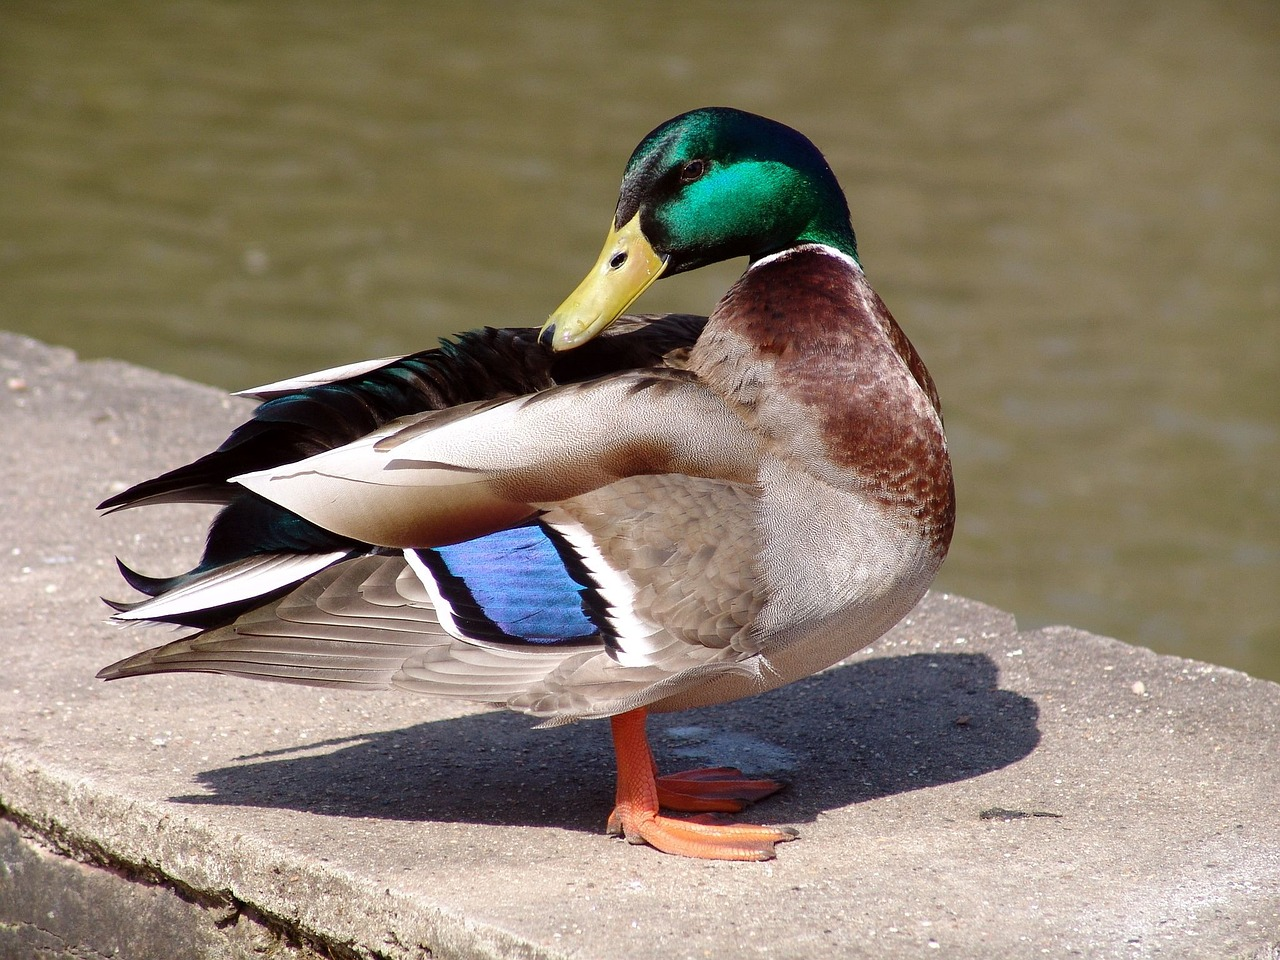
\includegraphics[width=\textwidth]{images/duck.jpg}


Da du aber wahrscheinlich ja eher Abbildungen machen willst versuche es hiermit.

\begin{figure}[h]
	\centering
	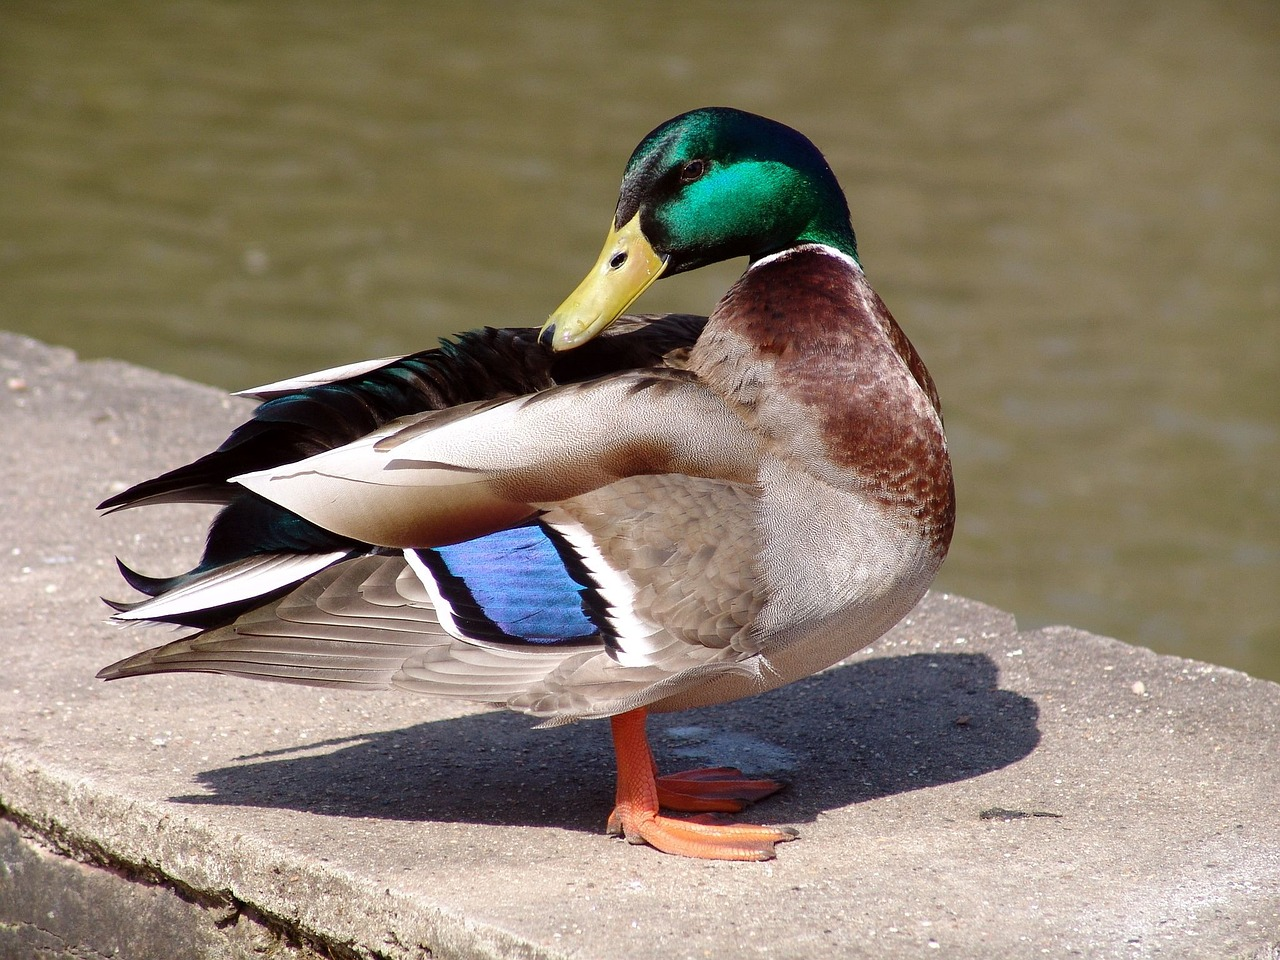
\includegraphics[width=0.7\textwidth]{images/duck.jpg}
	\caption{This is a smaller duck}
	\label{fig:duck}
\end{figure}
%\newpage
\section{Structure and Size of the Dataset} \label{sec:dataUnderstanding}

% minimum 1 page

The data used in the remainder of this paper \todo{"in this paper" -> vorher haben wir ja auch schon über die Daten gesprochen}comes from four individual datasets collected at different universities (Zurich, Budapest, Long Beach, Cleveland). The distribution of the target variable can be seen in \cref{table:datasets}.
% PLACEHOLDER TABLE
\begin{table}[h]

    \begin{footnotesize}
        \begin{tabular}{|l|l|l|l|}
            \hline
            \textbf{Origin of data set}              & \textbf{\# of instances} & \textbf{Distribution target variable} \\ \hline
            Hungarian Institute of Cardiology, Budapest & 294                      & 106 / 188                             \\ \hline
            University Hospital, Zurich                 & 123                      & 115 / 8                               \\ \hline
            V.A. Medical Center, Long Beach             & 200                      & 149 / 51                              \\ \hline
            Cleveland Clinic Foundation, Cleveland      & 282                      & 125 / 157                             \\ \hline
        \end{tabular}
    \end{footnotesize}
    \begin{center}
        \centering
        Distribution = heart disease / no heart disease
    \end{center}
    \caption{Content of the dataset}
    \label{table:datasets}
\end{table}



For the purposes of this paper, the four datasets are considered as one coherent dataset consisting of 77 attributes (33 numeric, 42 categorical, 1 constant) and a total of 899 measurements.
The attributes can be divided into the following categories:
\begin{multicols}{2}
    \begin{itemize}
        \item Patient data
        \item Electrocardiogram
        \item Cardiac fluoroscopy
        \item Coronary angiograms
    \end{itemize}
\end{multicols}
The category of patient data includes characteristics such as \textit{age}, \textit{sex} or type of chest pain (\textit{cp}), whereas the category electrocardiogram includes various electrocardiographic information obtained during an exercise electrocardiogram like the peak blood pressure (\textit{tpeakbps}). Cardiac fluoroscopy contains all measurements obtained from a cardiac fluoroscopy, a medical measure that allows to see the flow of blood through vessels to evaluate the presence of blockages. An example for an attribute from this category is \textit{ca} which denotes the number of found major vessels. The last category is coronary angiograms, which contains the results of the examination of the same name. The main attribute of interest of this category is \textit{num} because it is the target variable that denotes whether a patient has a heart disease or not. In the raw data, patients without a heart disease are shown with a value of 0 for \textit{num}, while patients with heart disease are shown with a value  $\geq 1$.
An overview of all remaining attributes which were not named here is provided in our code documentation as well as the UCI Machine Learning Repository \citep{janosi1988}. In general, it is assumed that the collected values are of high quality, as they are the result of standardised medical measurement procedures, apart from the individual characteristics described by the patient, such as the location or type of pain. For this reason, it is assumed that a combination of the individual data sets is possible. This is also true because the measurements are not sorted in a certain way, neither in the individual data sets nor in the combined dataset.

The dataset contains dates for the conducting of the electrocardiogram and coronary angiograms. These dates are unevenly distributed over a period of 7 years. We consider these dates irrelevant because we assume that the date of an examination does not affect its outcome as the period is to short to show evolutionary or general health changes in the society. Therefore a time series analysis is not possible with this dataset.

Finally, the distribution of the different variables in the combined dataset was analysed. The target variable was found to be reasonably symmetrically distributed with 495 positive and 404 negative measurements, implying a disease prevalence of about 55.1\% of the examined patients. Non-representative distributions were also found, e.g. \textit{sex} is non-representatively distributed with 78\% males and 22\% females. The same applies to \textit{age}, which is distributed similarly to a normal distribution in the range 28 to 77.

While assuming a high quality of the existing values, we found that $30,8\%$ of all fields are lacking measurements. This is attributed to the fact that not all universities have carried out all measurements. For example the Cleveland subset lacks the location of chest pain. Some individual attributes in particular have many missing values like history of diabetes (\textit{dm}) with roughly 90\% missing values. Whereby only positive cases may have been entered here, since 95\% of all filled cells show a diabetes disease which again is not representative. Furthermore, when checking whether meanings of attributes and their contained values fit together, we observe some irregularities. For example, the values 0 for cholesterol (\textit{chol}) and blood pressure \textit{testbps} are not compatible with life. Therefore, it is assumed that these values are misreported non-surveys, which are dealt with in the following chapter Preprocessing.






%\newpage
\section{Preprocessing} \label{sec:preprocessing}

Preprocessing was approached in two steps. In the first step the dataset was prepared based on knowledge obtained in \cref{sec:dataUnderstanding} and further analysis. 
Secondly, the data was transformed with the help of various algorithms that are combined in a pipeline. 

\subsection{Data Preparation }
In the first step a custom loading function was implemented to put the four data sets into a usable format and harmonise known differences in encodings. In this step, the missing values marked \texttt{$-9$} were replaced by \texttt{NaN} and the target variable was binarised by replacing all values greater than 1 by 1, as the UCI does not describe how the different positive cases (\textit{num} $\geq 1$) differ.

After that irrelevant columns such as IDs, dates, constants, undescribed columns as well as irrelevant columns according to the UCI were removed. All of these columns are either not causally related to the presence of heart disease or cannot be examined for new patients because it is unknown what they measure. The feature \textit{pncaden} was also dropped because it is the sum of the binary variables  pain location, pain during exercise and relief on rest and therefore contains no additional information. 

After the removal 55 attributes remained and were used to train the first model. XGBoost was chosen for that because it natively can handle \texttt{NaN} values. The accuracy of a 10-fold cross validation without any tuning was 0.98. This result was unexpectedly good, which is why   the importance of the different features was analysed. It was found that the features belonging to the category of the coronary angiograms were serving as false predictors and therefore removed, leaving us with 45 remaining features. To validate that the removal hat the desired effect the cross validation was run again this time with an accuracy of 0.76 and a more reasonable distribution in the weights of the features.   

After irrelevant columns were dropped the remaining features were analysed for inconsistencies. Here it was found that \textit{thaltime} which describes the moment a measurement was taken during the exercise is sometimes larger than \textit{thaldur} which denotes the duration of the exercise. In this case \textit{thaltime} was replaced by \texttt{NaN} in all 17 instances. Another inconsistency was found between the maximum heart rate (\textit{thalach}) and the heart rate at rest (\textit{thalrest}). If the maximum heart rate was below the resting heart rate the maximum heart rate was replaced by \texttt{NaN} since the values were unusually small.

\begin{figure}[h]
	\centering
	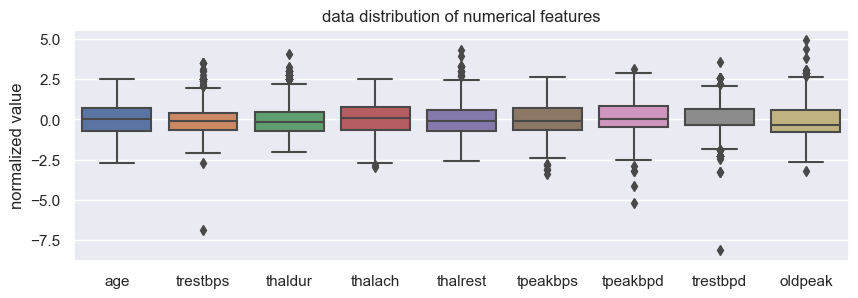
\includegraphics[width=\textwidth]{images/dataDistribution.png}
	\caption{data distribution of all numeric elements}
	\label{fig:dataDistribution}
\end{figure}
As shown in \cref{fig:dataDistribution}  normalised box plot of all numeric features were created to check for outliers. The features \textit{trestbps} and \textit{trestbpd} show extreme outliers with a value of 0. These are assumed to be incorrectly specified \texttt{NaN}s as stated in \cref{sec:dataUnderstanding} and are therefore replaced by \texttt{NaN}. All other outliers are not as extreme and come in groups. As the data contains sick persons, values diverging from the norm are expected. For these reasons it was decided to keep these outliers as they might be a strong indication of a heart disease.

After handling all errors in the dataset the categorical features \textit{cp, restecg, slope, ca, thal, restwm} were OneHotEncoded. All features were analysed regarding their pearson correlation, where only two pairs of features with a substantial amount of data ($<75\%$ \texttt{NaN}s) have a strong correlation ($>75\%$).  
These are asymptomatic chest pain $\leftrightarrow$ pain during exercise and \textit{rldv5} $\leftrightarrow$ \textit{rldv5e}. The first correlation seems plausible, as pain that only occurs under exercise is classified as asymptomatic. The features are still relevant, however, as the cases where there is no correlation are of particular interest. For \textit{rldv5} which denotes the height of the peak in the ECG during rest while \textit{rldv5e} is the same under exercise also the cases where there is no correlation are of special interest because this might be typical for people with a heart disease. In order to better understand the interrelationships two new features were computed. Both represent the difference between a peak and a resting measurement. Once for the ECG (\textit{rldv5\_diff}) and once for the blood pressure (\textit{thal\_diff}). 
Furthermore, the feature indicating whether a patient smokes was enhanced by using the number of cigarettes per day and the length of time a patient has been smoking to infer the boolean variable. Hereby, the number of \texttt{NaN}s was reduced from 74\% to 43\%. 

\subsection{Hyperparameter Tuning} \label{subsec:hyperparametertuning}
Additionally to the hyperparamter tuning of the estimators, which is described in \cref{sec:datamining}, the preprocessing steps were also optimised  by different hyperparameters.


Firstly, binning for the feature \textit{age} was added. Either 2, 5 bins or no binning at all are set as hyperparameters. The bins were encoded in an ordinal variable.

To impute the missing data a simple imputer was used. Missing values are replaced by the mean, median or mode of the feature. The KNN imputer was not used, because it is computationally much more expensive, while the iterative imputer is not used, as it is still experimental and therefore subject to change. Due to the high number of missing values and their uneven distribution across the features it was analysed how the number of imputed cells and number of features behave when columns with a certain amount of missing values are dropped. This is visualized in \cref{fig:percentageToBeDropped}.

\begin{figure}[h]
	\centering
	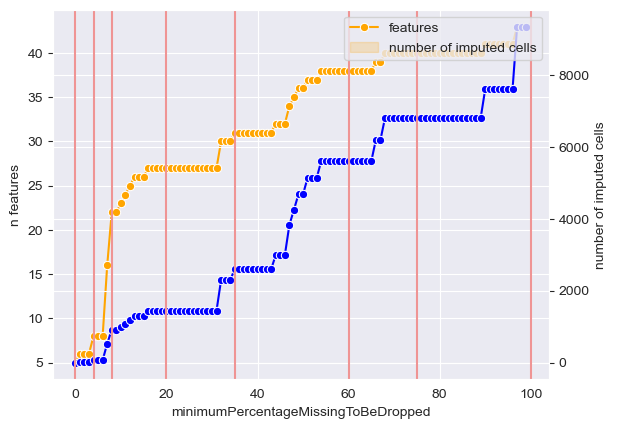
\includegraphics[width=\textwidth]{images/percentageToBeDropped.png}
	\caption{Number of features and values to be imputed by number of \texttt{NaN}s}
	\label{fig:percentageToBeDropped}
\end{figure}

It becomes apparent that there are certain steps where the number of features goes up a lot. To decide when a feature is included based on the number of missing values, the steps 0, 4, 8, 20, 35, 60, 75 and 100\% were set as hyperparameter. They are shown as vertical lines in the graph. 

To account for the different ranges of the features the MaxAbsScaler, MinMaxScaler, PowerTransformer, RobustScaler, Standardscaler and Normalizer are used. As the parameters of most scalers turn on or off core functionalities of the scaler, only tune the norm of the Normalizer was changed by hyperparameters with the norms l1, l2 and max.

To account for the slight imbalance of healthy and unhealthy patients oversampling and undersampling in the training data in comparison to no sampling was used. After this step the preprocessing is done. 


%The \textbf{MaxAbsScaler} scales the values of each feature by the maximum absolute value. Therefore, all values in [-1,1] can occur after scaling. \newline
%Using the \textbf{MinMaxScaler} results in values in [0,1] by shifting by the negative minimum and scaling by $maximum - minimum$\newline
%The values were normalized using the norms l1,l2 and max in the \textbf{Normalizer}. \newline
%The \textbf{PowerTransformer} alters the data to represent a gaußian like distribution. This is mostly used if heteroskedasticity occurs in the data. It was tried to fit the data to a standard normal distribution and without shifting and scaling by its mean and variance. \newline
%The \textbf{RobustScaler} was tried with and without scaling by the interquartile range and with and without shifting beforehand.\newline
%The \textbf{Standardscaler} was used with and without shifting by the mean and scaling by the standard deviation.\newline
%It was also tried, manly for comparison, to \textbf{passthrough} the values as they are.\newline
%\newpage
\section{Data mining} \label{sec:datamining}
The first step in the process of data mining is to decide on a fitting algorithm. Because the best algorithm is not known in advance multiple are tested. For this project these were: KNNeighbors, Random Forest, Decision Tree, SVC, logistic regression, XGBoost, and four naïve bayes classifiers based on bernoulli, complement, gaussian  and multinomial.

These ten classification algorithms will be evaluated to determine which one yields the best results. The quality of an algorithm is determined by two properties. The first criterion is a high recall, in order to avoid possible Type 2 errors (a patient with a heart disease is diagnosed as negative) in the diagnosis. The second criterion is the number of examinations required. The reason for this is that the model should be universally used by doctors. It is assumed that this is especially the case when simple examinations yield good diagnosis.

Besides the before mentioned use of scalers, imputers and samplers a variety of classifier specific hyperparameters were applied. For the KNN the number of used neighbors from 2 to 97 moving in 5-unit steps as well as the distance metric L1 and L2 as hyperparameters were added. The Random Forest was tested with 10 to 90 (10-unit steps) estimators and a maximum depth of None, 2, 6 and 10 and a minimum split of 2, 6, and 10. Decision Trees were tested with both the gini index and entropy as impurity measures while the values for maximum tree depth and minimum split were the same as for Random Forest. In the case of logistic regression, the same distance options as for KNN were added. For SVC C values ranging from 120 to 160 (20-unit steps), in combination with the gamma values 0.0001, 0.001, 0.01 and the kernel options linear, polynomial, sigmoidal and radial basis function were tested. For the four naïve bayes estimators alpha values from 0 to 19.5 (0.5-unit steps) were applied.

In order to find the best model a stratified nested cross validation was conducted using 10-folds each. To later decide which model was the best a classification report for every outer loop of the CV was saved. To run all CVs the work was split into several small parts where every unique combination of estimator, scaler and imputer represents its own part that was run on its own. In the following evaluation only the best model according to the previously defined criterions (high recall and simplicity) for each estimator is reviewed in greater detail. For measuring the simplicity the minimum percentage to be dropped was used as a metric. If models performed equally Occam's Razor was applied and favoured models with a low number of columns and basic preprocessing. The results without any ordering can be seen in \cref{table:modelresults} in addition to some further prediction metrics.


% INSERT TABLE

\begin{table}[h]
	\begin{adjustwidth}{-0.25cm}{}

	\begin{footnotesize}
		\begin{tabular}{|l|l|l|l|l|l|l|l|}
			\hline
			\textbf{Classifier} & \textbf{Scaler}  & \textbf{Sampler} & \textbf{Rec.} & \textbf{Rec. Std.} & \textbf{AUC.} & \textbf{F1} & \textbf{MPD} \\ \hline
			Baseline            & none             & none             & 1             & 0                  & 0.50         & 0.71        & 0            \\ \hline
			KNN                 & none             & none             & 0.85          & 0.04               & 0.76         & 0.80        & 0            \\ \hline
			XGB                 & Normalizer       & RUS              & 0.77          & 0.09               & 0.76         & 0.78        & 75           \\ \hline
			Random Forest       & StandardScaler   & none             & 0.84          & 0.09               & 0.78         & 0.81        & 100          \\ \hline
			Decision Tree       & none             & none             & 0.85          & 0.06               & 0.76         & 0.80        & 0            \\ \hline
			SVC                 & PowerTransformer & none             & 0.81          & 0.11               & 0.77         & 0.80        & 20           \\ \hline
			NB (bernoulli)      & StandardScaler   & none             & 0.79          & 0.08               & 0.76         & 0.79        & 8            \\ \hline
			NB (complement)     & MinMaxScaler     & none             & 0.84          & 0.03               & 0.77         & 0.81        & 100          \\ \hline
			NB (gaussian)       & Normalizer       & none             & 0.52          & 0.12               & 0.70         & 0.64        & 20           \\ \hline
			NB (multinomial)    & MinMaxScaler     & none             & 0.79          & 0.06               & 0.76         & 0.79        & 100          \\ \hline
			logistic regression & Normalizer       & none             & 0.84          & 0.07               & 0.76         & 0.80        & 0            \\ \hline
		\end{tabular}

		 \begin{adjustwidth}{+0.25cm}{}
		\begin{center}
			\centering
			RUS = random under sampler, MPD = minimum percentage to be dropped
		\end{center}
		\end{adjustwidth}
	\end{footnotesize}
	\caption{Best models for every classification algorithm}
	\label{table:modelresults}

	 \end{adjustwidth}
\end{table}

The table includes all estimators as well as the baseline (majority vote). 
As the majority vote predicts a disease in all cases there are no false negatives and therefore the recall of the baseline is always 1. However, the model would not be usable in the real world because the doctors would not benefit from the prediction as the model would predict the same for every patient. This is why the table also includes AUC and F1 as comparison, where the trained models outperform the baseline. This makes all models better to use than the baseline, as they can provide real added value. 

In order to find the best model first the recall is analyzed. Here larger differences can be observed. But the best performing models all have a recall of 0.84 to 0.85 (KNN, Random Forest, Descision Tree, NB (complete), logistic regression).  To further narrow down the selection, the simplicity of the models is considered on the basis of the MPD. Here the Random Forest and the NB model are excluded as they use all columns compared to the other models which only use completely filled columns. Since the remaining models do not differ significantly, a LeaveOneGroupOut cross validation is performed. Here, three data sets are used as the basis for training in order to classify the content of the fourth. The results for this procedure are also all within 0.01 for recall (0.78), precision (0.72), F1 (0.76), and accuracy (0.72). So they are assumed to be equal and Occam's Razor is conducted once more. KNN and the Decision Tree are simpler in preprocessing compared to the Logistic regression as they both do not use a scaler. If KNN and the Decision Tree are compared in their simplicity the Decision Tree outperforms the KNN because medical staff can just follow the Decision Tree whereas a KNN computation can not be done easily. 
So it is argued that the best model for classifying whether somebody has a heart disease or not is the model which uses the Decision Tree, followed closely by the before discussed KNN and logistic regression models.


The Decision Tree uses no scaler nor sampler. Also, no imputer was used because MPD is 0 and therefore no features with missing values remain. The best configuration was gini index as purity measure, a maximum tree depth of \texttt{None} and a minimum split of 2. This is identical to the defaults set by scikit-learn. 
In order to view what the model assumes to be important indicators it is visualized in \cref{fig:DecisionTree}. Only  the tree with depth 3 (total depth 5) is displayed since focus is on the main attributes. 
\begin{figure}[h]
	\centering
	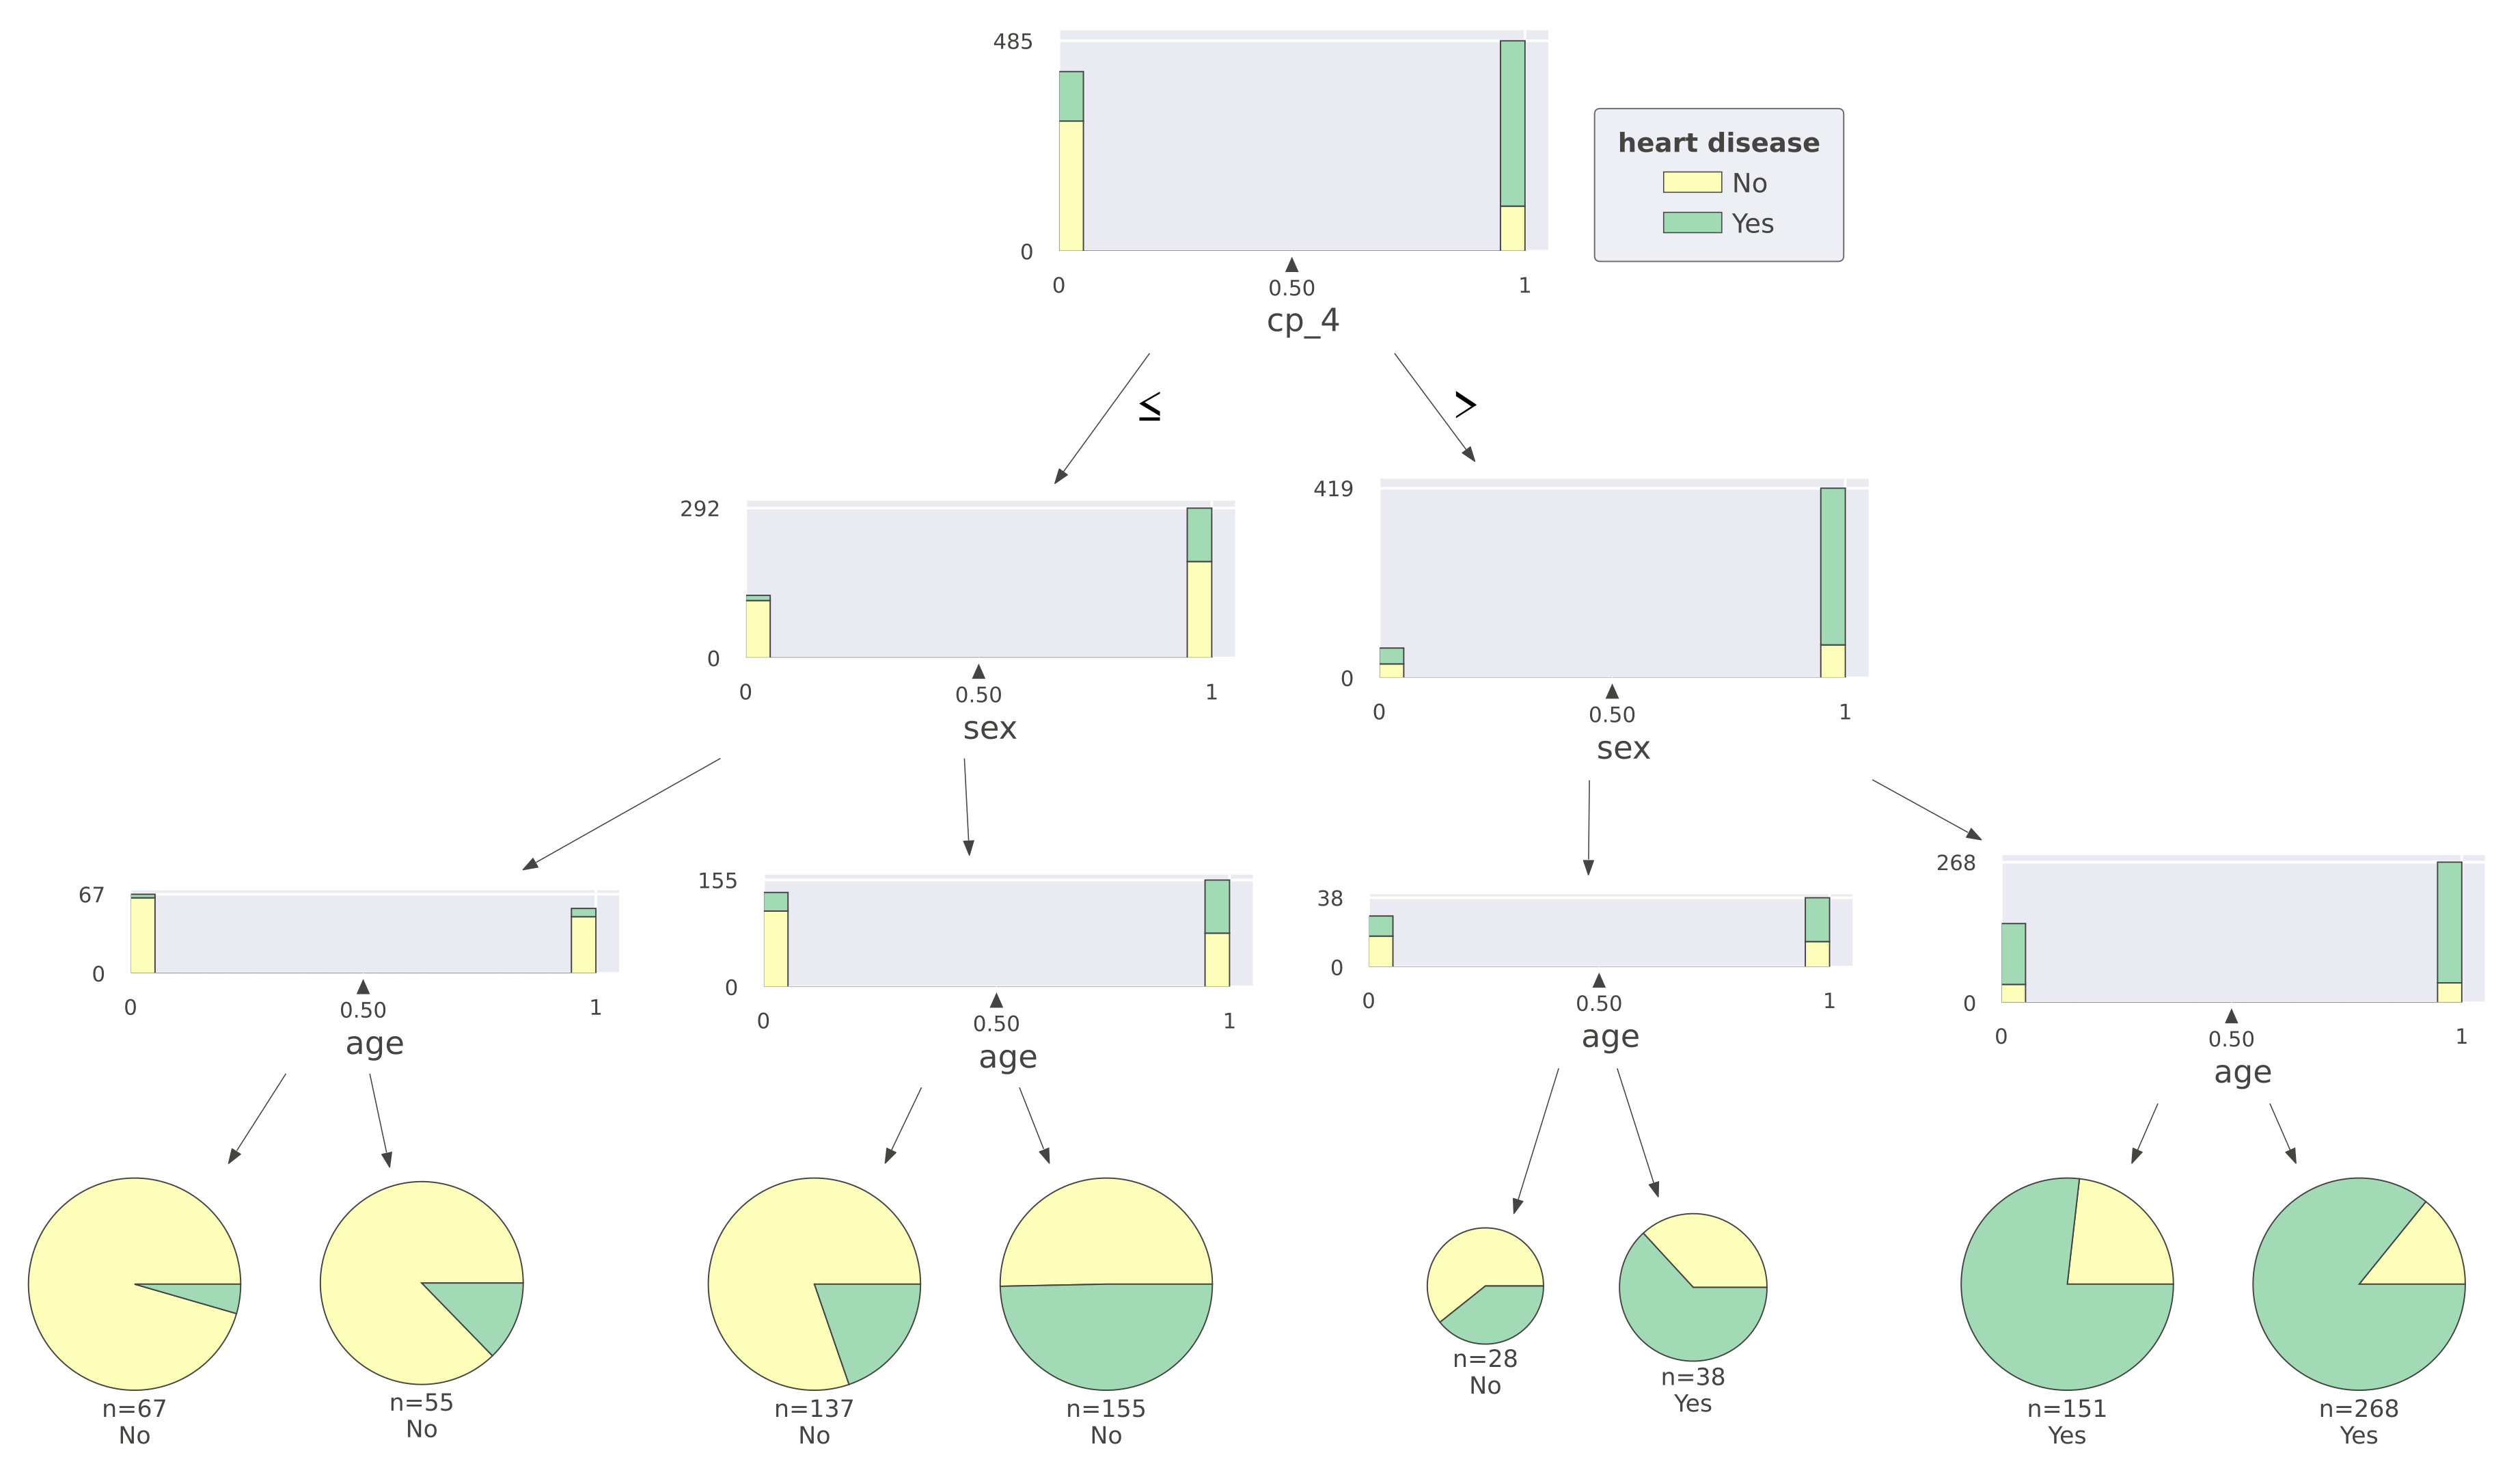
\includegraphics[width=0.7\textwidth]{images/DecisionTree.png}
	\caption{Decision Tree visualized}
	\label{fig:DecisionTree}
\end{figure}

The root node of the tree decides whether a participant had asymptomatic chest pain or not. The resulting follow-up nodes both use gender as the next split criterion. After that the tree splits according to age. The visualization shows that older men with asymptomatic chest pain have the highest chance to be predicted to have a heart disease. Overall, the model predicts men of all ages and with or without asymptomatic chest pain to have a higher probability of having a heart disease compared to women. The group with the lowest chance of having a heart disease are young women with no asymptomatic chest pain. The left side of the cp split conducts two more splits based on cp that are not displayed here. 


%\newpage
\section{Results} \label{sec:results}

In order to be able to critically assess the result with the decision tree as the best model, a comparison is made with existing evaluations. Therefore, a search for papers, articles and competitions working with the dataset which describe their approach well is conducted. In doing so,  it became clear that the used approach is not widespread. The dataset is frequently used, but not as a whole. Often only one sub-dataset, mostly Cleveland, is used.  In comparison to the works that work exclusively on the Cleveland dataset, our best model is surpassed in every respect (\cite{Ayatollahi2019,alotaibi2019, uyar2017}). It should be noted that other models might not be generalisable as the models in this paper, as they may represent noise from the respective data set. Furthermore, it should be noted that the Cleveland dataset is a very pure dataset compared to the other datasets and hardly contains any missing values. 
A comparison of the most important features is also not possible as the only work that that used every feature also included the false predictors in their models \cite{garate-escamila2020}.

When compareing the best model against the majority class baseline with a recall of 1, the best model is surpassed. Though this is manly due to the poor selection of recall as key metric as it does not reflect the usefulness of the model because it ignores the performance on negative values. If F! is used as a metric the Decision tree is able to outperform the baseline. 

To conclude whether the project helps doctors on diagnosing possible heart diseases more easily, certain limitations into needed to be taken into account. Type 2 errors in disease prediction are particularly problematic because a sick patient is mistakenly found to be healthy and therefore might not receive the correct treatment. Contrary the Type 1 error, might lead to healthy patients getting medication they do not need.   When considering the actual application of the model in practice, it is important to overcome the "black box" of machine learning for users. For this, explainable AI models like the Decision Tree help to be interpretable and trustworthy even for laymen (see \cref{fig:DecisionTree}). Therefore, the Decision Tree is a well chosen model. Though the decisions made by the Tree (old man with asymptomatic chest pain are likely to have a heart disease) is well known for years. Therefore, applying the model in the real world would not make sense as there is no added value for the user. 

% =============================================
% 			END OF CONTENT!
% =============================================


\newpage
\printbibliography

%\vspace{2cm}
%\begin{small}
  %\printbibliography
  % \printbibliography[title = {Quellenverzeichnis}] To use a different name
%\end{small}

\pagestyle{plain}

\end{document}
